\subsection{Tilbagekobling}
\label{effekt_tilbagekobling}
For at regne på tilbagekoblingen til effektforstærkeren er det nødvendigt at kende open-loop forstærkningen, $A$, som er givet ved udtrykket vist i formel (\ref{equ:a-openloop}).

\begin{equation}
\label{equ:a-openloop}
A = A_\mathrm{diff.amp} \cdot A_\mathrm{vol.amp} \cdot A_\mathrm{cur.amp}
\end{equation}

Spændingsforstærkningen i differensforstærkeren, $A_\mathrm{diff.amp}$, er i afsnit \ref{effekt_differensforstaerker} fundet til XXXXXX, mens spændingsforstærkningen i spændingsforstærkeren, $A_\mathrm{vol.amp}$, i afsnit \ref{effekt_spaendingsforstaerker} er fundet til XXXXXX. Spændingsforstærkningen i strømforstærkeren, som er en common-collector, $A_\mathrm{cur.amp}$, er givet ved udtrykket i formel (\ref{equ:a-cc})\fixme{kilde: formel 4.96 i sedra smith}, hvor $R_L$ er belastningsmodstanden på 8 \ohm~ i serie med den termiske sikringsmodstand på 0,536 \ohm~ og $r_e$ er en T-model-parameter.

\begin{equation}
\label{equ:a-cc}
A_\mathrm{cur.amp} = \frac{R_L}{R_L+r_e}
\end{equation}

T-model-parameteren $r_e$ er givet ved udtrykket i formel (\ref{equ:beta-re})\kilde{afsnit 4.5.7 i sedra smith}.

\begin{equation}
\label{equ:beta-re}
r_e = \frac{\alpha}{g_m} = \frac{\alpha}{\frac{I_C}{V_T}}
\end{equation}

Transistorparameteren $\alpha$ er givet ved udtrykket i formel (\ref{equ:alpha-def}).

\begin{equation}
\label{equ:alpha-def}
\alpha = \frac{\beta}{\beta + 1}
\end{equation}

Det ses af udtrykket i formel (\ref{equ:alpha-def}) at $\alpha \approx 1$, da $\beta>>1$ for BDX33B og BDX34B. Dermed kan $r_e$, for en $I_C$ på de maksimale 2,24 A, bestemmes som vist i formel (\ref{equ:beta-re1}).

\begin{equation}
\label{equ:beta-re1}
r_e \approx \frac{1}{\frac{\mathrm{2,24~A}}{\mathrm{26~mA}}} \approx \mathrm{11,6~m\ohm}
\end{equation}

Resultatet i udregningen i formel (\ref{equ:beta-re1}) leder til en bestemmelse af $A_\mathrm{cur.amp}$ som vist i beregningen i formel (\ref{equ:a-cc-val}).

\begin{equation}
\label{equ:a-cc-val}
A_\mathrm{cur.amp} = \frac{\mathrm{8,536~\ohm}}{\mathrm{8,536~\ohm~} + \mathrm{11,6~m\ohm}} = 0,99
\end{equation}

Open-loop forstærkningen, $A$, kan nu bestemmes som vist i udregningen i formel (\ref{equ:a-openloop-val}).

\begin{equation}
\label{equ:a-openloop-val}
A = A_\mathrm{diff.amp} \cdot A_\mathrm{vol.amp} \cdot A_\mathrm{cur.amp} = XXXXXX \cdot XXXXXX \cdot 0,99 = XXXXXX
\end{equation}

Closed-loop forstærkningen, $A_f$, som er givet ved udtrykket vist i formel (\ref{equ:af_def})\kilde{formel 9.4 i sedra smith}, ønskes til 8,95. Dette skyldes at der, som beregnet i afsnit \ref{valg_kortslutningssikring}, skal være 17,9 V over belastningen når der kommer 2 V som input til effektforstærkeren.

\begin{equation}
\label{equ:af_def}
A_f = \frac{A}{1 + A \cdot \beta}
\end{equation}

Da $A$ er bestemt i formel (\ref{equ:a-openloop-val}), kan $\beta$ ud fra udtrykket i formel (\ref{equ:af_def}) bestemmes til XXXXXX. Med $\beta$ fastlagt, kan mængden af tilbagekobling bestemmes som vist i udregningen i formel (\ref{equ:amountfeedback}).

\begin{equation}
\label{equ:amountfeedback}
1 + A \cdot \beta = XXXXXX
\end{equation}

Tilbagekoblingskredsløbet opbygges som en spændingsdeler, som vist på figur \ref{fig:beta-clean}, hvormed closed-loop forstærkningen, $A_f$, bliver som vist i formel (\ref{equ:af-deler})\kilde{eksempel 9.1 i sedra smith}.

\begin{figure}[h]
\centering
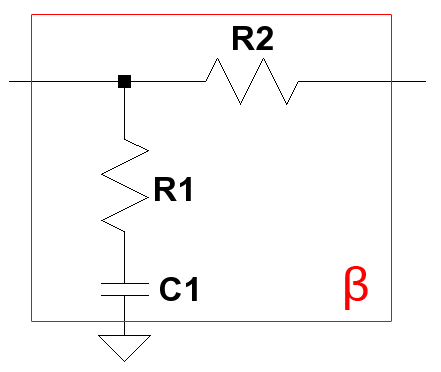
\includegraphics[scale=0.4]{teknisk/effektforstaerker/beta-clean.png}
\caption{Opbygning af tilbagekoblingskredsløb}
\label{fig:beta-clean}
\end{figure} 

\begin{equation}
\label{equ:af-deler}
A_f = \frac{R_1 + R_2}{R_1} = 1 + \frac{R_2}{R_1}
\end{equation}

Dette er gældende så længe $A \cdot \beta >> 1$, hvilket er tilfældet. For at opnå en $A_f$ på 8,95 skal forholdet mellem $R_2$ og $R_1$ altså være 7,95. Kondensatoren, $C_1$, er indsat for at tilbagekoble hele DC-signalet. Dette sker da kondensatoren er en afbrydelse for DC

\subsubsection*{Simulering}